\documentclass[aspectratio=1610]{beamer}

\usetheme{KTH}
\usepackage{preamble}

% Advice from Schule, that was given to him as advice when he was becoming a researcher.
%
% Three thirds, 1 third for everybody, 1 third for experts, and 1 third for yourself to show off.

% ====>>>>> general

%% The slides should be for the audience, to give them a visual experience.
%% Transitions; one style for the slides and one style for the transitions between topics. e.g. light background, dark text vs. dark background, light text.
%% Don't write too much on the slides.
%% Skip effects.
%% Masking images to direct attention.
%% Simple charts and graphs. If possible, in the same style as the presentation (e.g. fonts, colors).

\begin{document}

% === [ Start page ] ===========================================================

\startpage

\begin{frame}
	\vspace{0.02\textheight}

	\begin{Large}
		Evaluation of Methods for Effective Control Flow Recovery
	\end{Large}

	\vspace{0.1\textheight}

	\begin{small}
		\textit{Robin Eklind}
	\end{small}
\end{frame}

% === [ Disposition ] ==========================================================

\normalpage

\begin{frame}
	\frametitle{Disposition}

	\begin{enumerate}
		\item What? \textit{Control Flow Recovery}
		\item Why? \textit{Applications of Control Flow Recovery}
		\item How? \textit{Control Flow Recovery Methods}
		\item Technical Contributions
		\item Future Work
		\item Demo!
	\end{enumerate}
\end{frame}


% === [ Introduction ] =========================================================

% ====>>>>> What?

% What?

% Frame problem at a high level.
% 1-3 minutes.

% Key message you wish to communicate. From the perspective of the audience, what will they gain? What can they do with the information?

\begin{frame}
	\frametitle{What?}

	\begin{block}{Control Flow Recovery}
		Analysis of control flow graphs (CFGs) to recover high-level control flow primitives (e.g. \texttt{if}-statement and \texttt{for}-loops) from assembly or low-level intermediate representations.
	\end{block}
\end{frame}

\begin{frame}
	\frametitle{Control Flow Recovery}

	\begin{figure}[htbp]
		\centering
		\begin{subfigure}[t]{0.27\textwidth}
			\centering
			\lstinputlisting[caption={C source file.}, language=C, style=c, basicstyle=\tiny\ttfamily, breaklines=false, numbers=none]{inc/overview/overview.c}
		\end{subfigure}
		\quad
		\begin{subfigure}[t]{0.52\textwidth}
			\centering
			\lstinputlisting[caption={LLVM IR assembly.}, language=llvm, style=nasm, basicstyle=\tiny\ttfamily, breaklines=false, numbers=none]{inc/overview/overview_mini.ll}
		\end{subfigure}
		\caption{\textit{Reverse compilation}, going from low-level (right) to high-level (left).}
	\end{figure}

\end{frame}

% ====>>>>> Why?

% Why?

% Then go into depth; both intellectual and emotional arguments for the severity of the problem.
% 15-20 minutes if presenting for 1 hour.

\begin{frame}
	\frametitle{Why?}

	\begin{block}{Applications of Control Flow Recovery}
		\begin{itemize}
			\item Malware analysis
			\item Security assessments
			\begin{itemize}
				\item Automated vulnerability scanning
			\end{itemize}
			\item Control-flow aware compiler passes
			\item Verification of compiler output (\textit{Reflections on Trusting Trust})
			\item Reverse compilation
			\begin{itemize}
				\item Transpilation between programming languages ($n + m$)
				\item Migrate proprietary software from legacy architectures
				\item Re-optimization of software where source code or tool chain is missing
			\end{itemize}
% Note to speaker: For Cobol.
%   - semantic equivalence, with a lot of goto-s to begin.
%   - clean up over time.
		\end{itemize}
	\end{block}
\end{frame}

\begin{frame}
	\frametitle{Control-flow Aware Compiler Passes}

	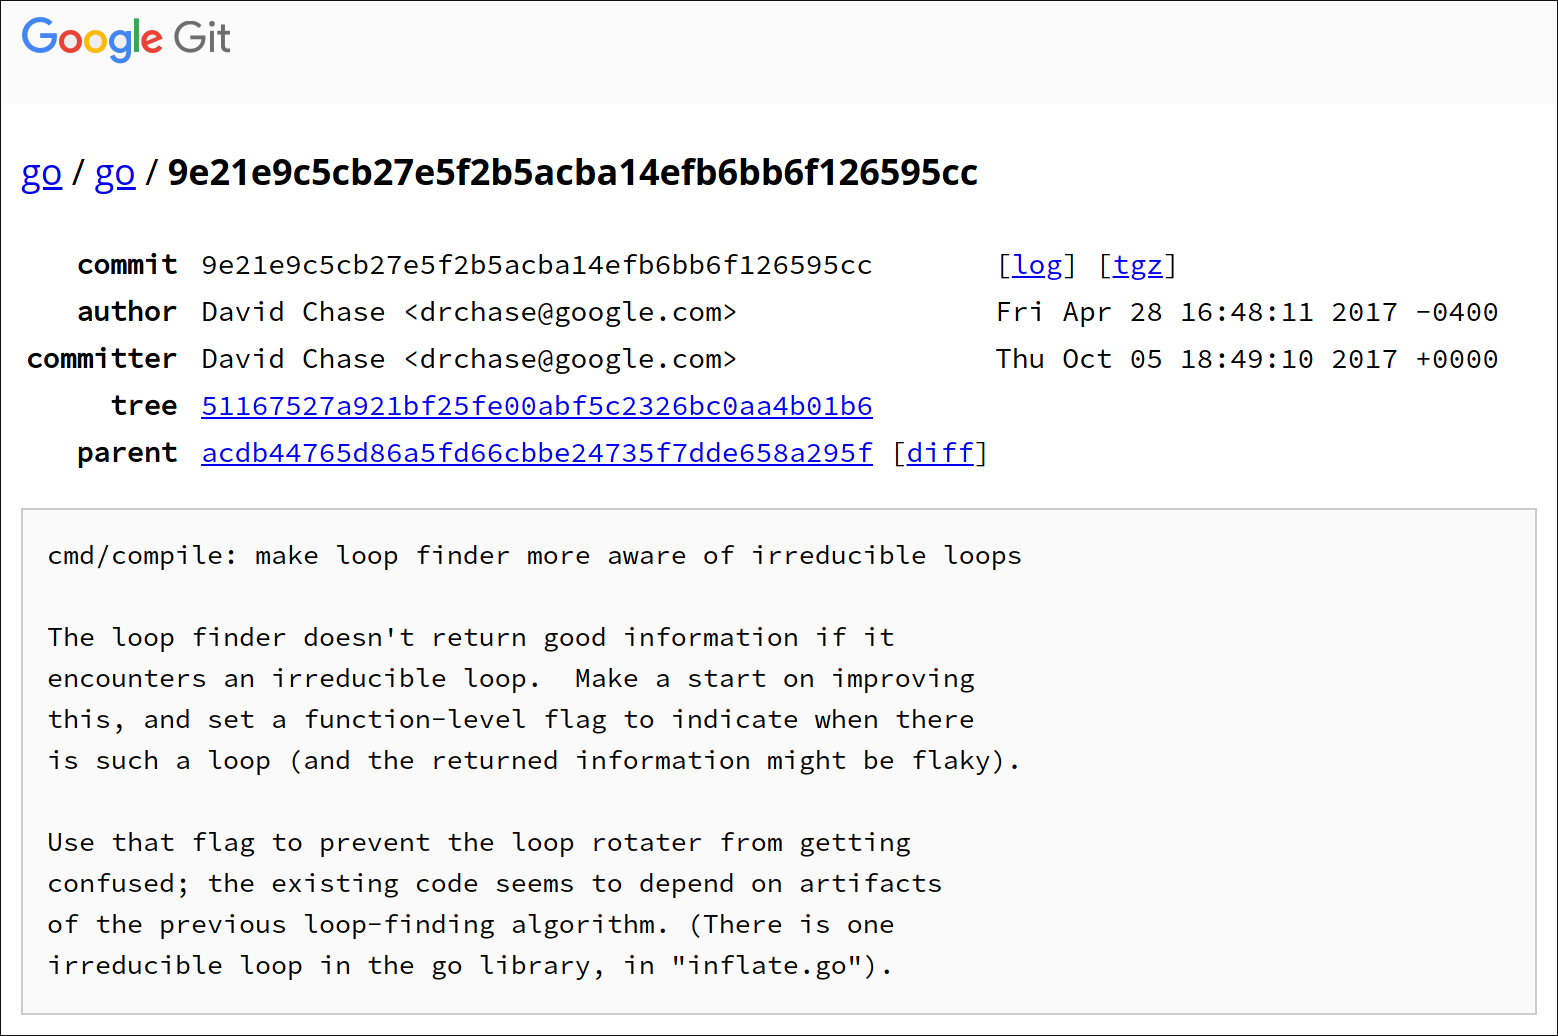
\includegraphics[width=0.8\textwidth]{inc/applications/loop_finder.png}
\end{frame}

\begin{frame}
	\frametitle{Issues with State-of-the-Art Reverse Compilation Tools}

	\begin{figure}[htbp]
		\centering
		\begin{subfigure}[ht]{0.30\textwidth}
			\centering
			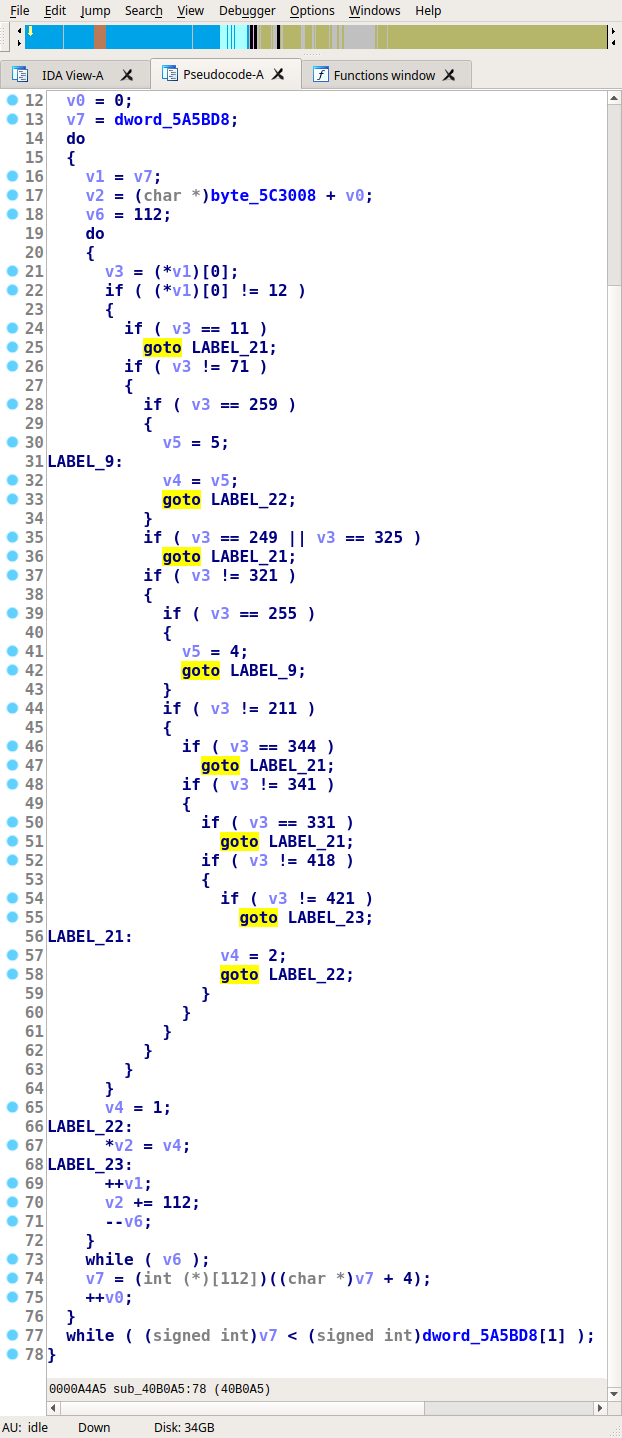
\includegraphics[height=0.80\textheight]{inc/applications/ida/ida_40B0A5.png}
		\end{subfigure}
		\begin{subfigure}[ht]{0.40\textwidth}
			\centering
			\lstinputlisting[caption={Corresponding Go source code.}, language=go, style=go, basicstyle=\tiny\ttfamily, breaklines=false, numbers=none]{inc/applications/ida/go_40B0A5.go}
		\end{subfigure}
		% IDA Version 7.1.180227
		\caption{IDA output (left) and corresponding Go source code (right).}
	\end{figure}
\end{frame}

% ====>>>>> How?

% How?

% Give solution, including benefits and drawbacks.

\begin{frame}
	\frametitle{How?}

	\begin{block}{Control Flow Recovery Methods}
		\begin{itemize}
			\item Hammock method
			\item Interval method
			\item Pattern-independent method
		\end{itemize}
	\end{block}

	There are benefits and drawbacks with each method.
\end{frame}

% --- [ Hammock method ] -------------------------------------------------------

\begin{frame}
	\frametitle{Hammock method}

	Model high-level control flow primitives as subgraphs and use \textit{subgraph isomorphism search} to locate the corresponding subgraphs in CFGs.

	\vspace*{2em}

	\begin{block}{Pros}
		\begin{itemize}
			\item \textit{no} false positives
		\end{itemize}
	\end{block}

	\begin{block}{Cons}
		\begin{itemize}
			\item \textit{many} false negatives
			\item requires single-entry/single-exit invariant for subgraphs
		\end{itemize}
	\end{block}

\end{frame}

\begin{frame}
	\frametitle{Hammock method}

% One example for each method, how it works.

	\begin{figure}[htbp]
		\centering
		\begin{subfigure}[b]{0.20\textwidth}
			\centering
			\lstinputlisting[language=C, style=c, basicstyle=\tiny\ttfamily, breaklines=false, numbers=none]{inc/methods/hammock/example/if.c}
			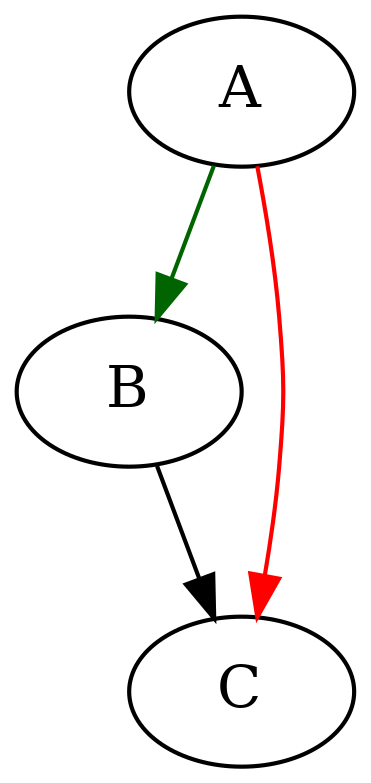
\includegraphics[width=0.4\textwidth]{inc/methods/hammock/example/if.png}
			\caption{Cannonical 1-way conditional.}
		\end{subfigure}
		\quad
		\begin{subfigure}[b]{0.65\textwidth}
			\centering
			\begin{subfigure}[ht]{0.40\textwidth}
				\centering
				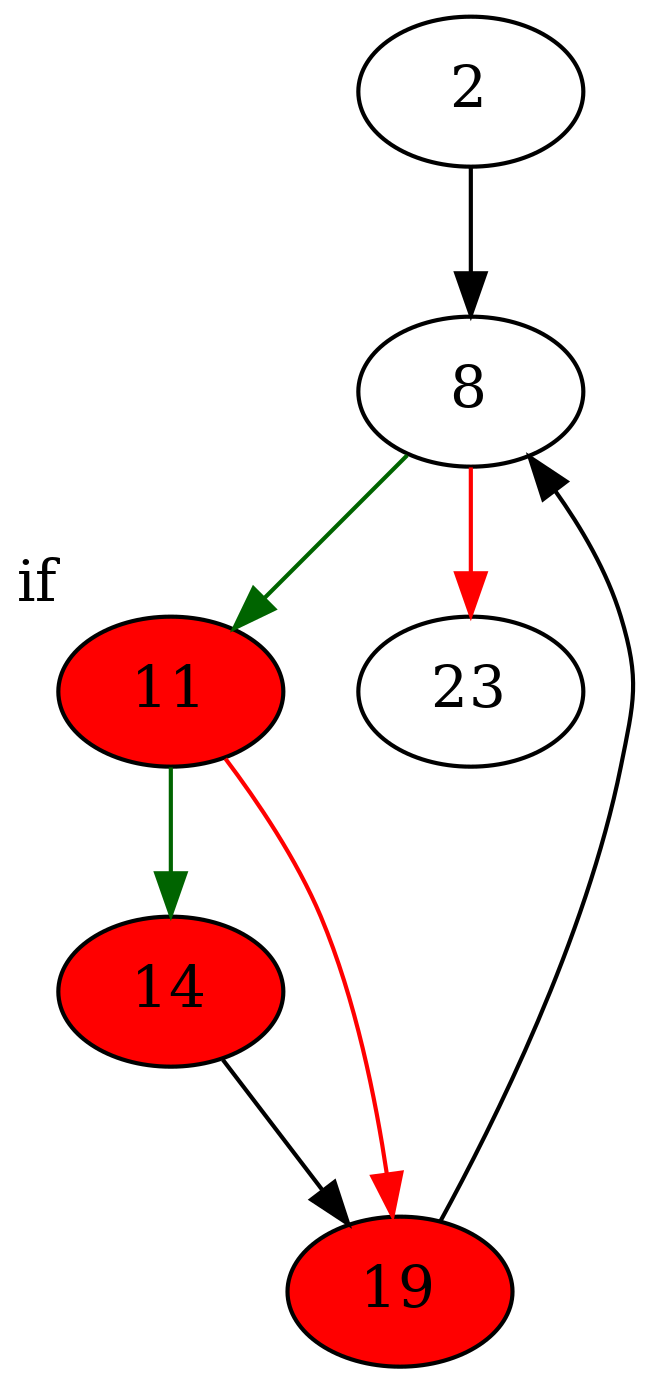
\includegraphics[width=0.5\textwidth]{inc/methods/hammock/example/main_0002a.png}
			\end{subfigure}
			\quad
			\begin{subfigure}[ht]{0.40\textwidth}
				\centering
				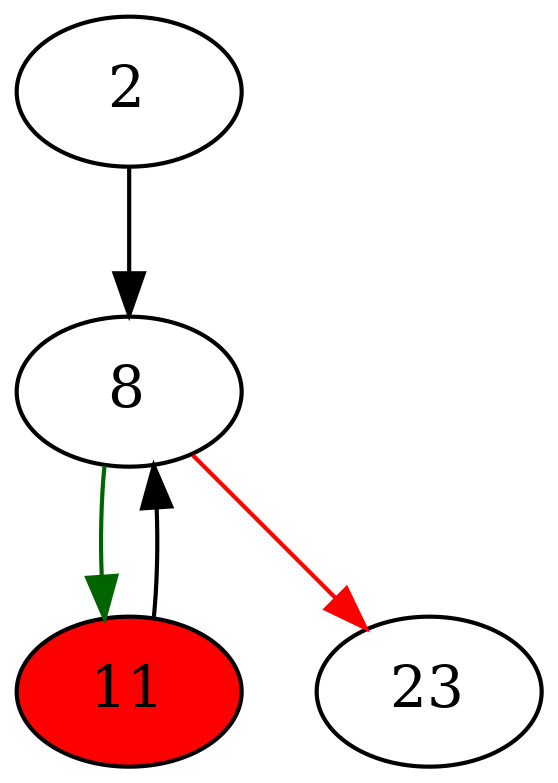
\includegraphics[width=0.5\textwidth]{inc/methods/hammock/example/main_0002b.png}
			\end{subfigure}
			\caption{Subgraph isomorphism of cannonical 1-way conditional located in control flow graph (left) and its nodes merged (right).}
		\end{subfigure}
	\end{figure}
\end{frame}

% ___ [ Hammock - Example ] ____________________________________________________

\begin{frame}
	\frametitle{Hammock method - example}
	\begin{figure}[htbp]
		\centering
		\begin{subfigure}[b]{0.30\textwidth}
			\centering
			\lstinputlisting[language=C, style=c, basicstyle=\tiny\ttfamily, breaklines=false]{inc/methods/hammock/example/without-break.c}
			\caption{Original C source code.}
		\end{subfigure}
		\begin{subfigure}[b]{0.50\textwidth}
			\centering
			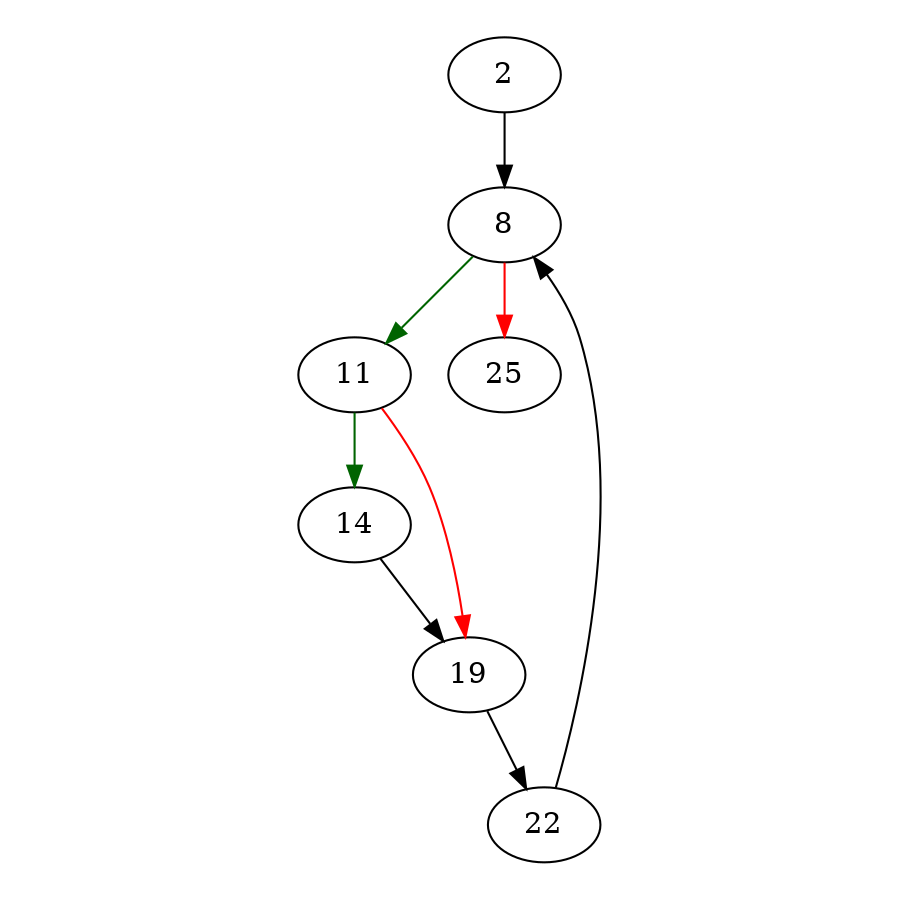
\includegraphics[height=0.6\paperheight]{inc/methods/hammock/example/without-break/main.png}
			\caption{Control flow graph.}
		\end{subfigure}
	\end{figure}
\end{frame}

\begin{frame}
	\frametitle{Hammock method - example}
	\begin{figure}[htbp]
		\centering
		\begin{subfigure}[b]{0.30\textwidth}
			\centering
			\lstinputlisting[linebackgroundcolor={\btLstHL{9-10}}, language=C, style=c, basicstyle=\tiny\ttfamily, breaklines=false]{inc/methods/hammock/example/without-break.c}
			\caption{Original C source code.}
		\end{subfigure}
		\begin{subfigure}[b]{0.50\textwidth}
			\centering
			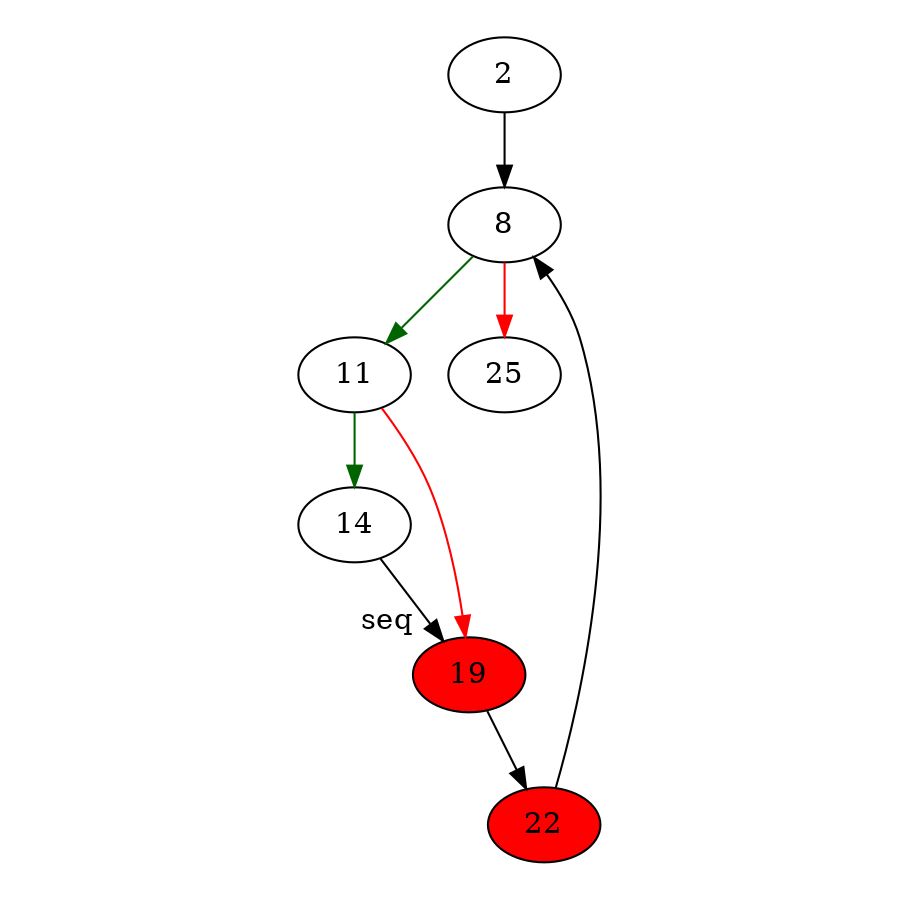
\includegraphics[height=0.6\paperheight]{inc/methods/hammock/example/without-break/main_0001a.png}
			\caption{Control flow graph.}
		\end{subfigure}
	\end{figure}
\end{frame}

\begin{frame}
	\frametitle{Hammock method - example}
	\begin{figure}[htbp]
		\centering
		\begin{subfigure}[b]{0.30\textwidth}
			\centering
			\lstinputlisting[linebackgroundcolor={\btLstHL{9-10}}, language=C, style=c, basicstyle=\tiny\ttfamily, breaklines=false]{inc/methods/hammock/example/without-break.c}
			\caption{Original C source code.}
		\end{subfigure}
		\begin{subfigure}[b]{0.50\textwidth}
			\centering
			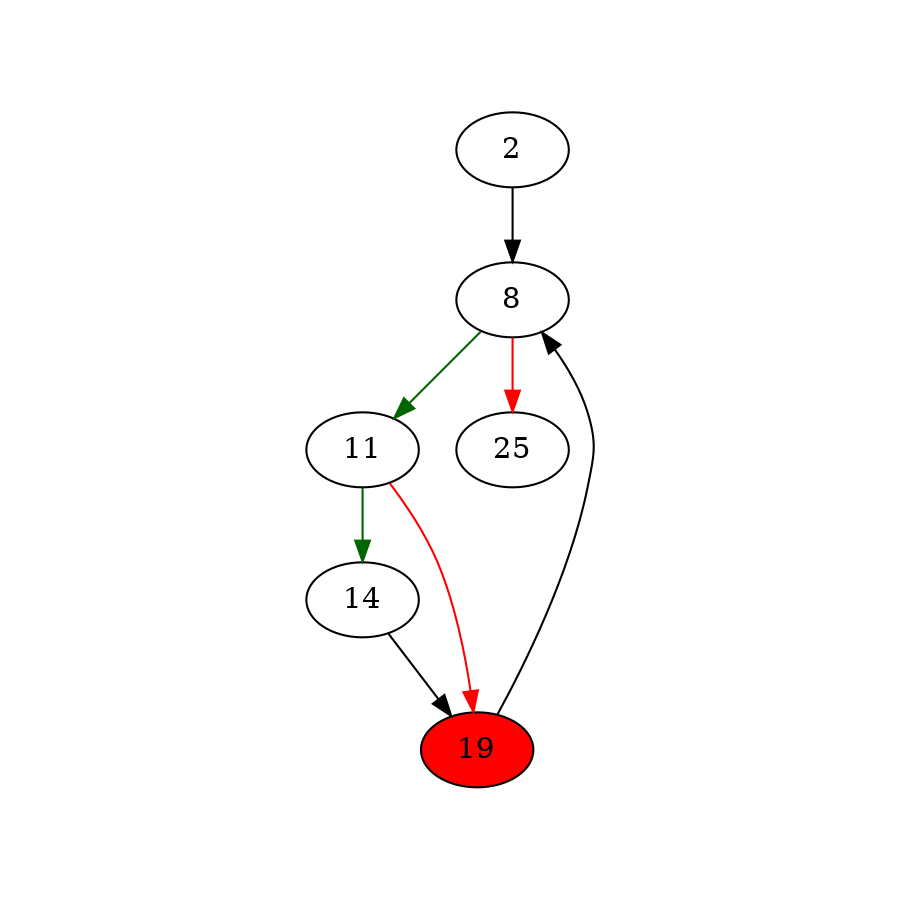
\includegraphics[height=0.6\paperheight]{inc/methods/hammock/example/without-break/main_0001b.png}
			\caption{Control flow graph.}
		\end{subfigure}
	\end{figure}
\end{frame}

\begin{frame}
	\frametitle{Hammock method - example}
	\begin{figure}[htbp]
		\centering
		\begin{subfigure}[b]{0.30\textwidth}
			\centering
			\lstinputlisting[linebackgroundcolor={\btLstHL{6-8}}, language=C, style=c, basicstyle=\tiny\ttfamily, breaklines=false]{inc/methods/hammock/example/without-break.c}
			\caption{Original C source code.}
		\end{subfigure}
		\begin{subfigure}[b]{0.50\textwidth}
			\centering
			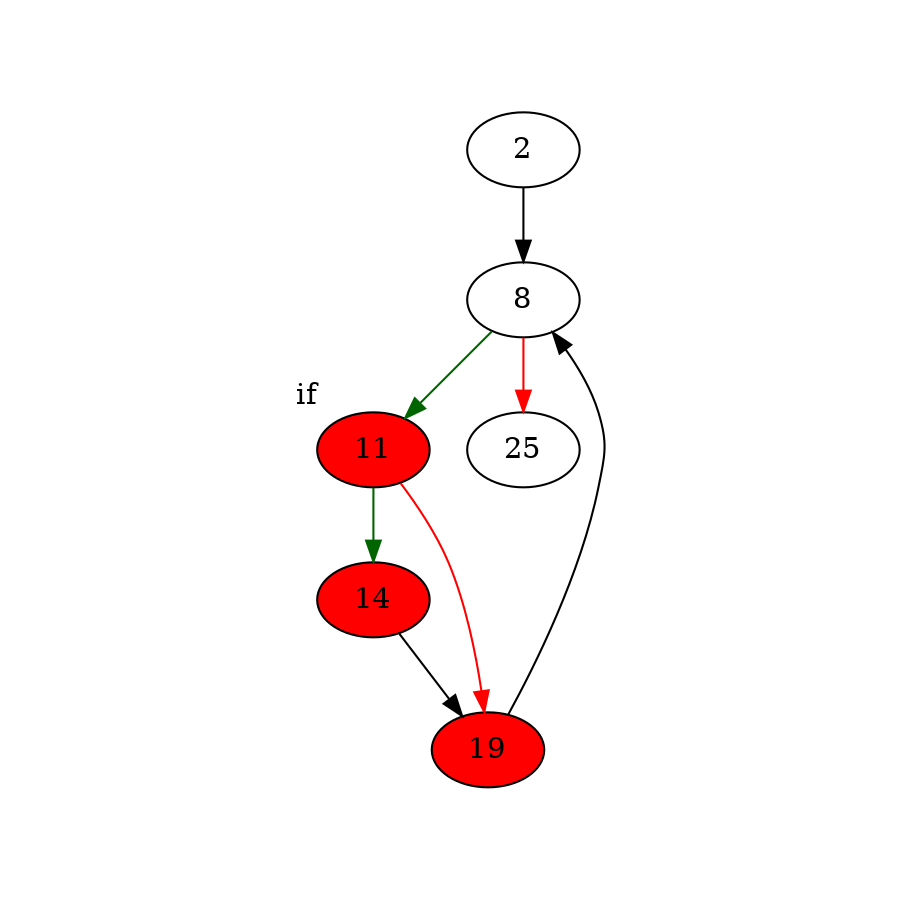
\includegraphics[height=0.6\paperheight]{inc/methods/hammock/example/without-break/main_0002a.png}
			\caption{Control flow graph.}
		\end{subfigure}
	\end{figure}
\end{frame}

\begin{frame}
	\frametitle{Hammock method - example}
	\begin{figure}[htbp]
		\centering
		\begin{subfigure}[b]{0.30\textwidth}
			\centering
			\lstinputlisting[linebackgroundcolor={\btLstHL{6-8}}, language=C, style=c, basicstyle=\tiny\ttfamily, breaklines=false]{inc/methods/hammock/example/without-break.c}
			\caption{Original C source code.}
		\end{subfigure}
		\begin{subfigure}[b]{0.50\textwidth}
			\centering
			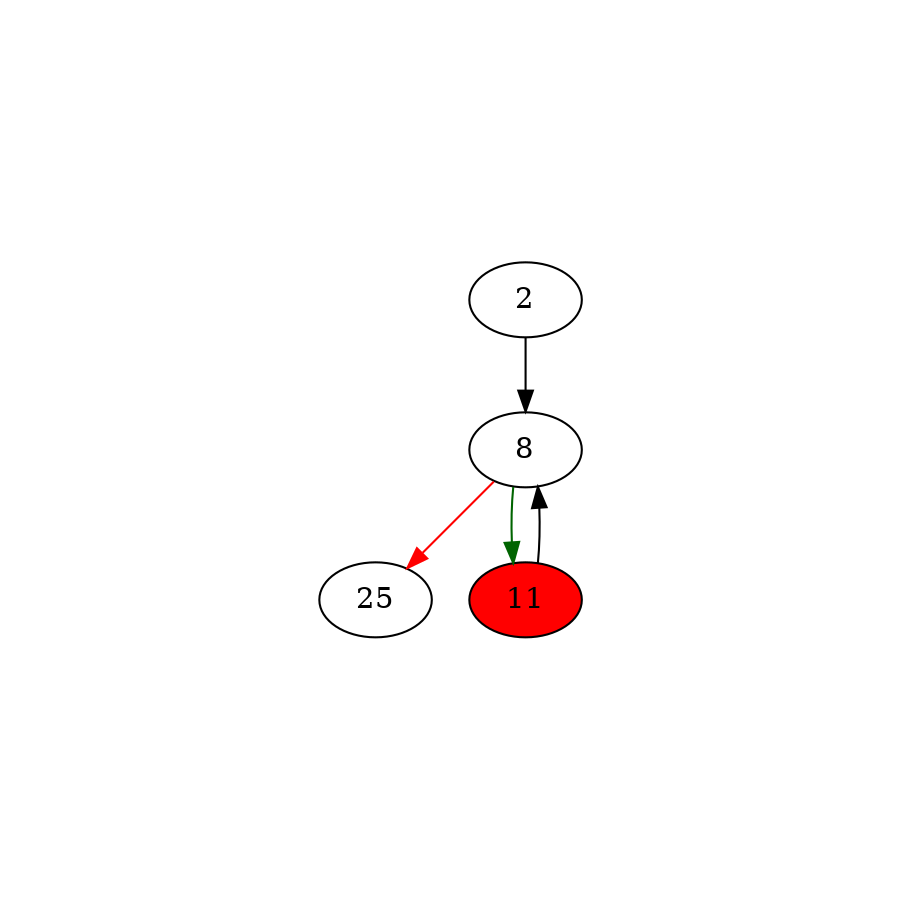
\includegraphics[height=0.6\paperheight]{inc/methods/hammock/example/without-break/main_0002b.png}
			\caption{Control flow graph.}
		\end{subfigure}
	\end{figure}
\end{frame}

\begin{frame}
	\frametitle{Hammock method - example}
	\begin{figure}[htbp]
		\centering
		\begin{subfigure}[b]{0.30\textwidth}
			\centering
			\lstinputlisting[linebackgroundcolor={\btLstHL{5, 10}}, language=C, style=c, basicstyle=\tiny\ttfamily, breaklines=false]{inc/methods/hammock/example/without-break.c}
			\caption{Original C source code.}
		\end{subfigure}
		\begin{subfigure}[b]{0.50\textwidth}
			\centering
			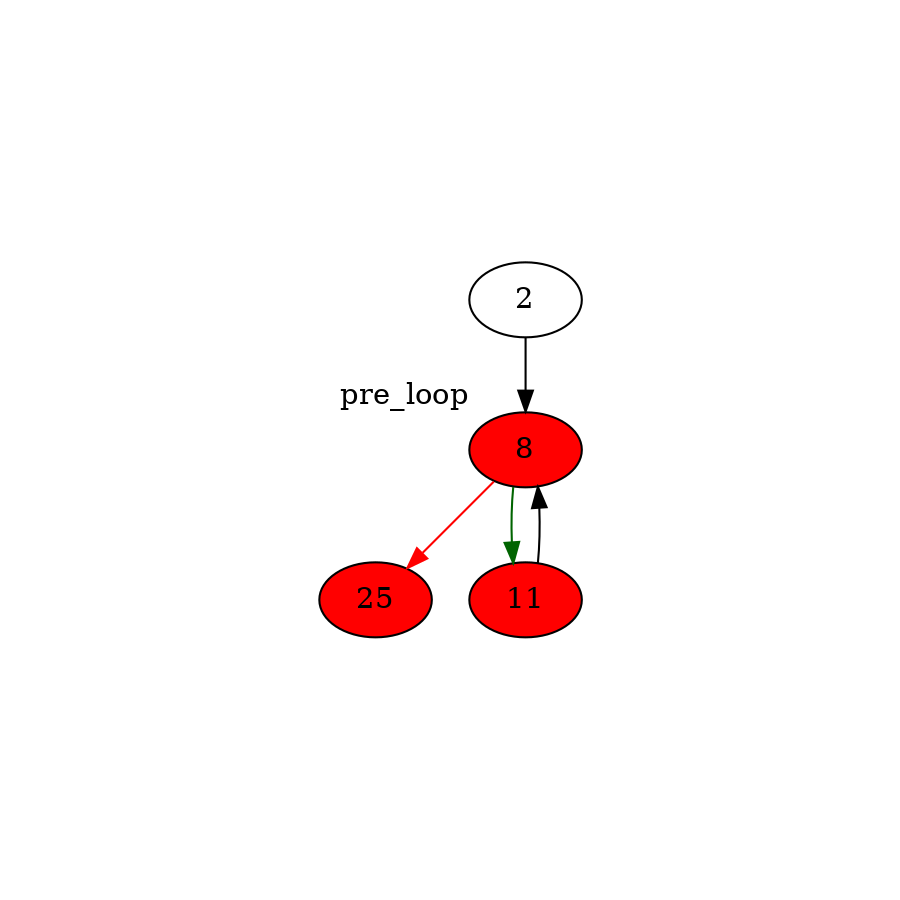
\includegraphics[height=0.6\paperheight]{inc/methods/hammock/example/without-break/main_0003a.png}
			\caption{Control flow graph.}
		\end{subfigure}
	\end{figure}
\end{frame}

\begin{frame}
	\frametitle{Hammock method - example}
	\begin{figure}[htbp]
		\centering
		\begin{subfigure}[b]{0.30\textwidth}
			\centering
			\lstinputlisting[linebackgroundcolor={\btLstHL{5, 10}}, language=C, style=c, basicstyle=\tiny\ttfamily, breaklines=false]{inc/methods/hammock/example/without-break.c}
			\caption{Original C source code.}
		\end{subfigure}
		\begin{subfigure}[b]{0.50\textwidth}
			\centering
			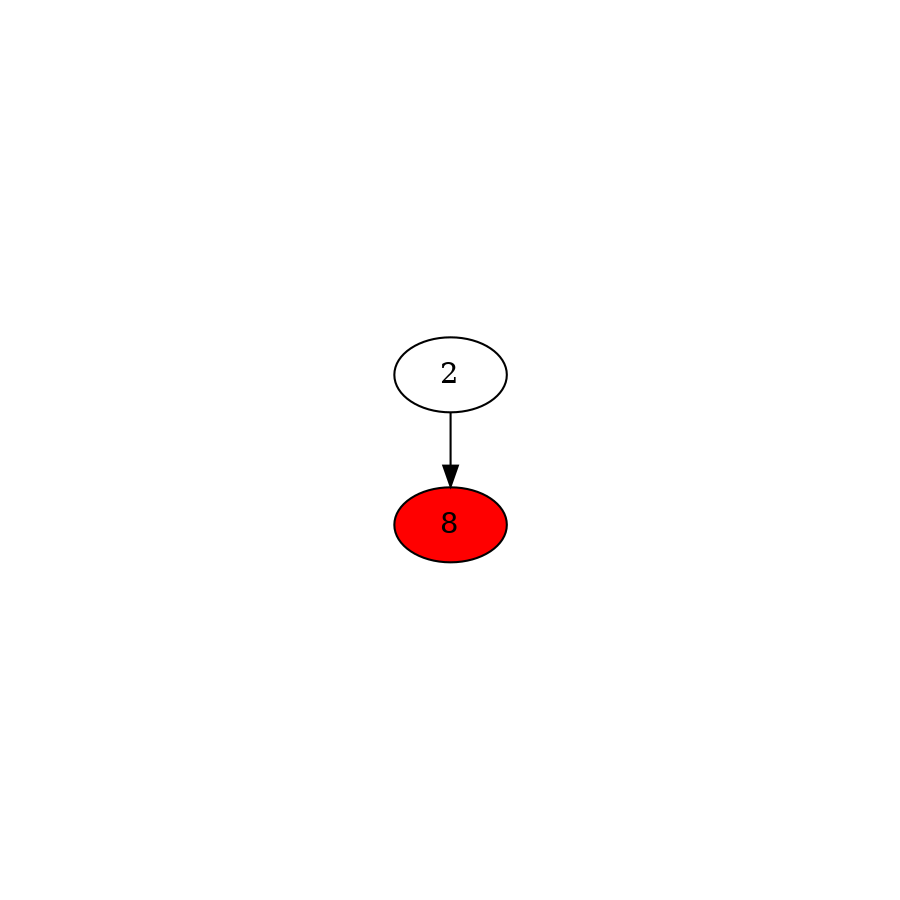
\includegraphics[height=0.6\paperheight]{inc/methods/hammock/example/without-break/main_0003b.png}
			\caption{Control flow graph.}
		\end{subfigure}
	\end{figure}
\end{frame}

\begin{frame}
	\frametitle{Hammock method - example}
	\begin{figure}[htbp]
		\centering
		\begin{subfigure}[b]{0.30\textwidth}
			\centering
			\lstinputlisting[linebackgroundcolor={\btLstHL{2-4}}, language=C, style=c, basicstyle=\tiny\ttfamily, breaklines=false]{inc/methods/hammock/example/without-break.c}
			\caption{Original C source code.}
		\end{subfigure}
		\begin{subfigure}[b]{0.50\textwidth}
			\centering
			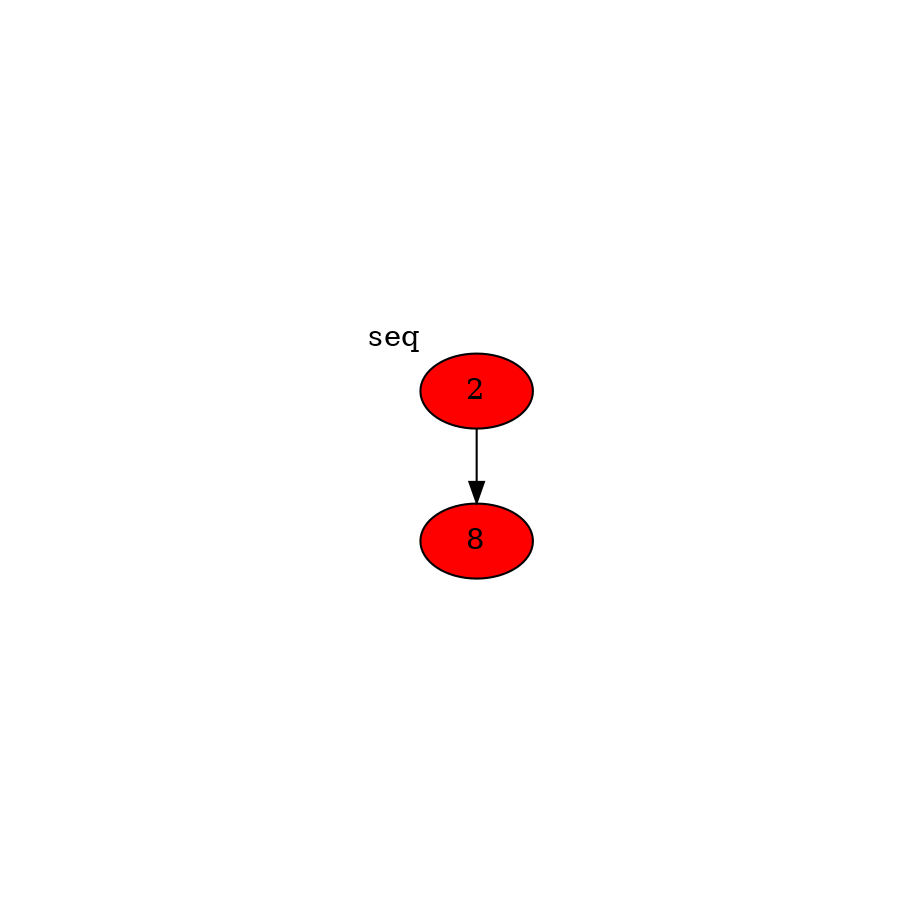
\includegraphics[height=0.6\paperheight]{inc/methods/hammock/example/without-break/main_0004a.png}
			\caption{Control flow graph.}
		\end{subfigure}
	\end{figure}
\end{frame}

\begin{frame}
	\frametitle{Hammock method - example}
	\begin{figure}[htbp]
		\centering
		\begin{subfigure}[b]{0.30\textwidth}
			\centering
			\lstinputlisting[linebackgroundcolor={\btLstHL{2-4}}, language=C, style=c, basicstyle=\tiny\ttfamily, breaklines=false]{inc/methods/hammock/example/without-break.c}
			\caption{Original C source code.}
		\end{subfigure}
		\begin{subfigure}[b]{0.50\textwidth}
			\centering
			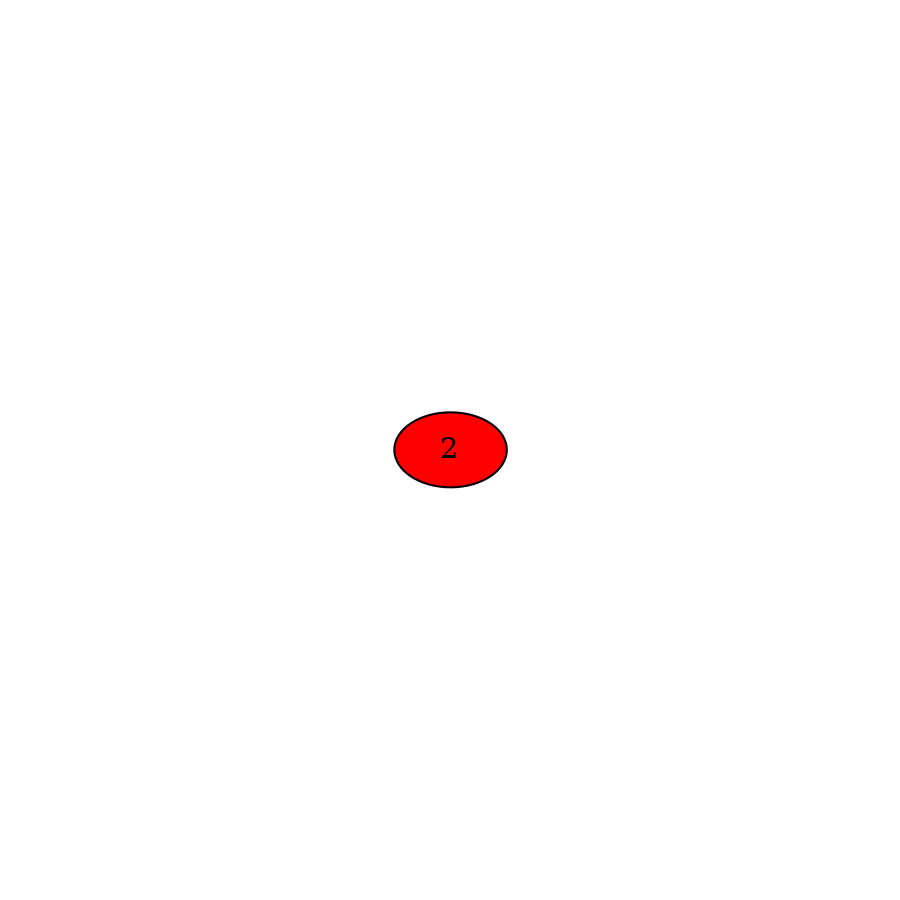
\includegraphics[height=0.6\paperheight]{inc/methods/hammock/example/without-break/main_0004b.png}
			\caption{Control flow graph.}
		\end{subfigure}
	\end{figure}
\end{frame}

% ___ [ Hammock - Counter-example ] ____________________________________________

% One example for each method, counter-example when it doesn't work.

\begin{frame}
	\frametitle{Hammock method - counter-example}
	\begin{figure}[htbp]
		\centering
		\begin{subfigure}[b]{0.50\textwidth}
			\centering
			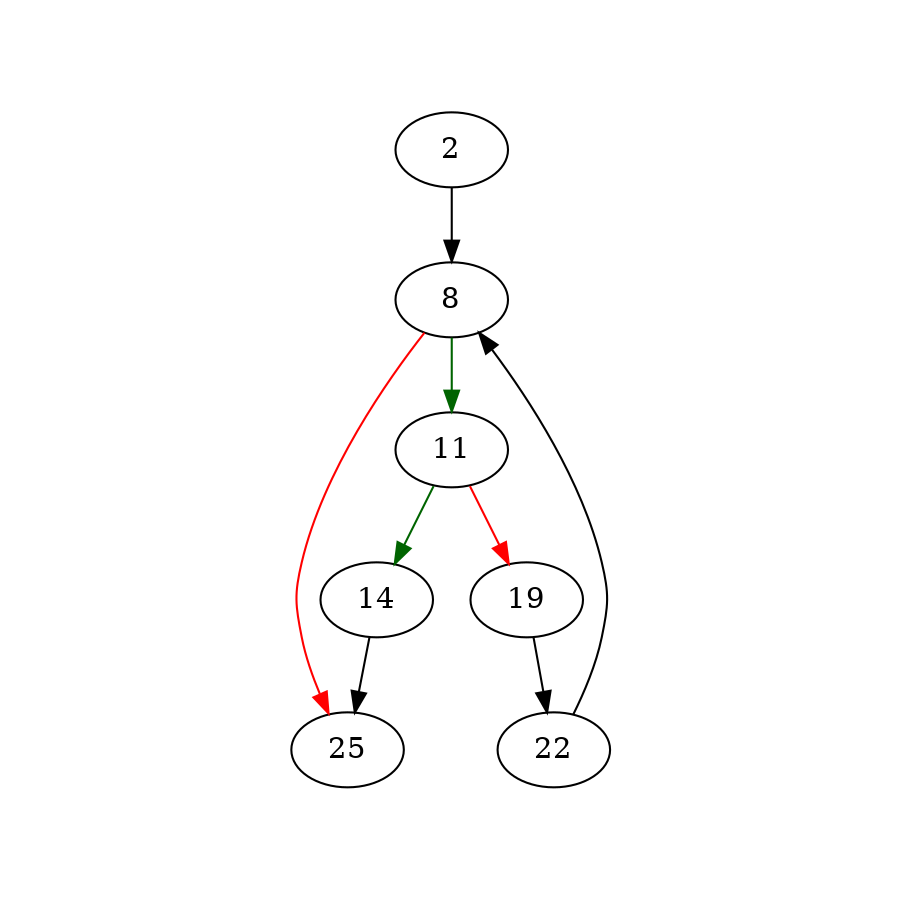
\includegraphics[height=0.6\paperheight]{inc/methods/hammock/counter-example/with-break/main.png}
		\end{subfigure}
	\end{figure}
\end{frame}

\begin{frame}
	\frametitle{Hammock method - counter-example}
	\begin{figure}[htbp]
		\centering
		\begin{subfigure}[b]{0.50\textwidth}
			\centering
			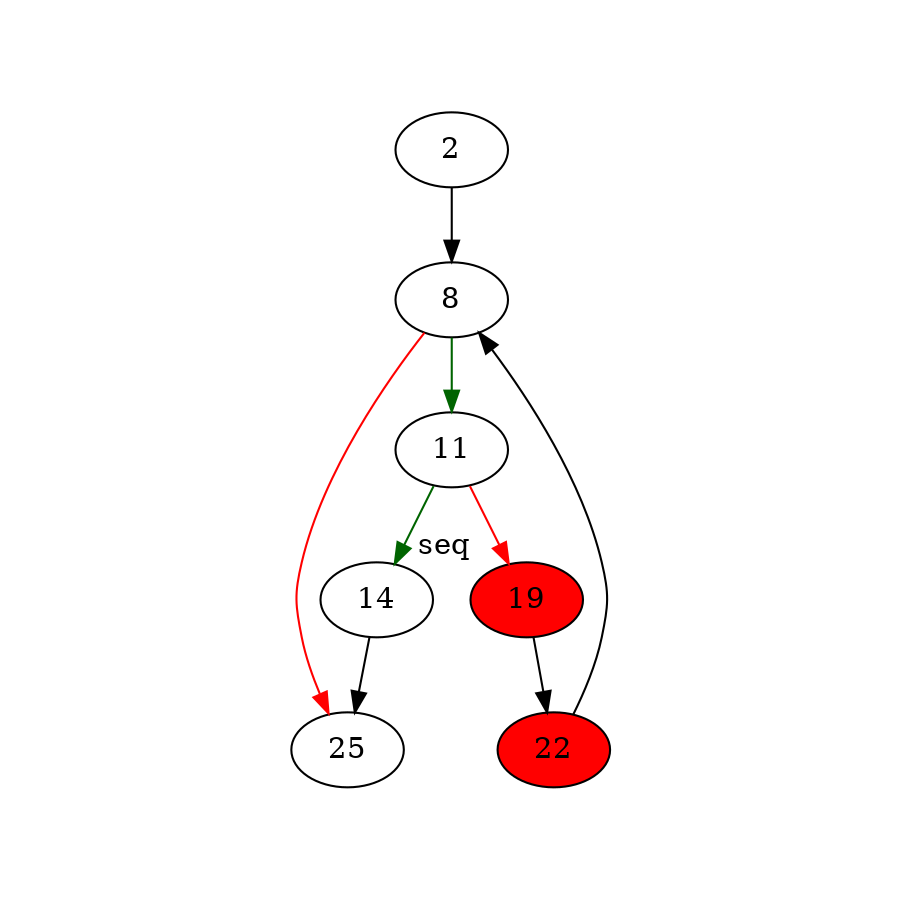
\includegraphics[height=0.6\paperheight]{inc/methods/hammock/counter-example/with-break/main_0001a.png}
		\end{subfigure}
	\end{figure}
\end{frame}

\begin{frame}
	\frametitle{Hammock method - counter-example}
	\begin{figure}[htbp]
		\centering
		\begin{subfigure}[b]{0.50\textwidth}
			\centering
			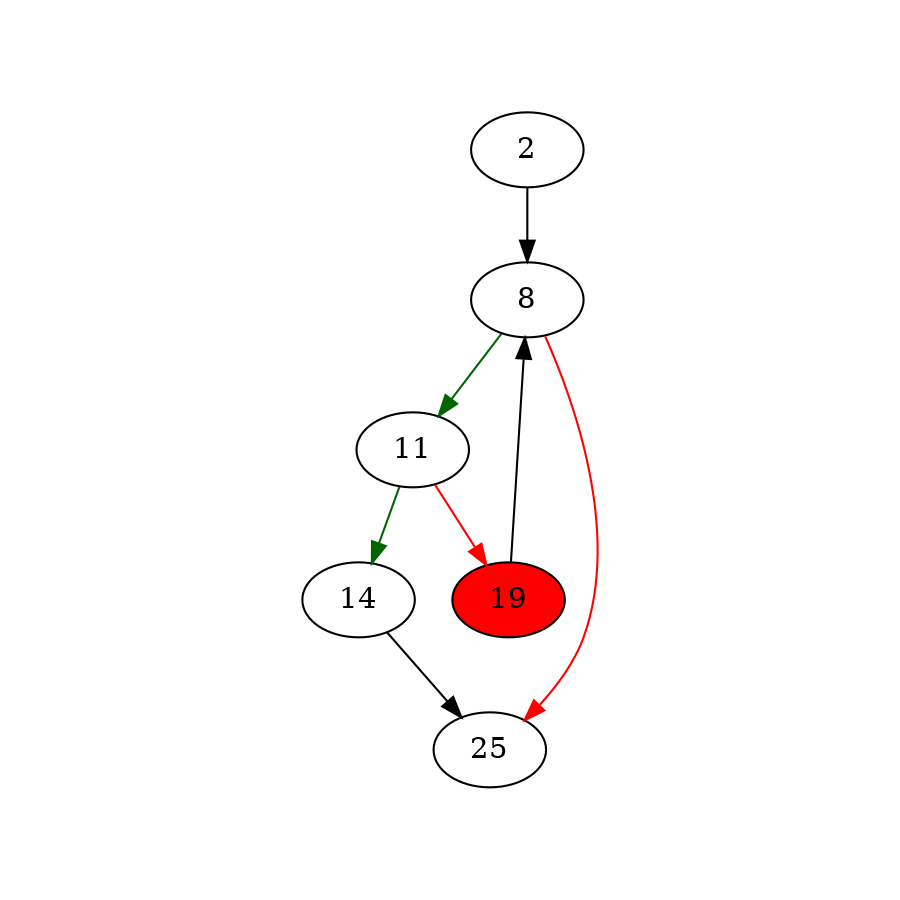
\includegraphics[height=0.6\paperheight]{inc/methods/hammock/counter-example/with-break/main_0001b.png}
		\end{subfigure}
	\end{figure}
\end{frame}

% --- [ Interval method ] ------------------------------------------------------

\begin{frame}
	\frametitle{Interval method}

	Identify intervals in CFGs to determine follow sets of high-level control flow primitives.

	\vspace*{2em}

	\begin{block}{Pros}
		\begin{itemize}
			\item handles multi-level \texttt{continue}- and \texttt{break}-statements in loops
		\end{itemize}
	\end{block}

	\begin{block}{Pros/Cons}
		\begin{itemize}
			\item \textit{some} false positives
			\item \textit{some} false negatives
		\end{itemize}
	\end{block}

% solved by interval method:
% - multi-level break and continue of loops.

\end{frame}

\begin{frame}
	\frametitle{Interval method - example}

% TODO: One example for each method, how it works.
	TODO
\end{frame}

\begin{frame}
	\frametitle{Interval method - counter-example}

% TODO: One example for each method, counter-example when it doesn't work.
	TODO
\end{frame}

% --- [ Pattern-independent method ] -------------------------------------------

\begin{frame}
	\frametitle{Pattern-independent method}

	Considers the conditions required to reach a node in the CFG rather than modelling explicit patterns. Relies on semantic-preserving transformations to pre-process CFGs.

	\vspace*{2em}

	\begin{block}{Pros}
		\begin{itemize}
			\item \textit{no} false negatives
			\item \texttt{goto}-free output
		\end{itemize}
	\end{block}

	\begin{block}{Cons}
		\begin{itemize}
			\item \textit{many} false positives
			\item introduces auxiliary condition variables (not present in original source)
		\end{itemize}
	\end{block}

% solved by pattern-independent method:

%    if (a & !b) {
%       // code1
%    }
%    if (b) {
%       // code 2
%    }
%    if (!b) {
%       // code 3
%    }

%    if (a & !b) {
%       // code1
%       goto LABEL_1
%    }
%    if (b) {
%       // code 2
%    }
%    if (!b) {
%    LABEL_1:
%       // code 3
%    }

\end{frame}

\begin{frame}
	\frametitle{Pattern-independent method - example}

% TODO: One example for each method, how it works.
	TODO
\end{frame}

\begin{frame}
	\frametitle{Pattern-independent method - counter-example}

% TODO: One example for each method, counter-example when it doesn't work.
	TODO
\end{frame}

% === [ Technical Contributions ] ==============================================

\begin{frame}
	\frametitle{Technical Contributions}

% TODO: Description of what I did, and what I achieved.
	TODO

\end{frame}

% === [ Future Work ] ==========================================================

\begin{frame}
	\frametitle{Future Work}

% TODO: speculations.

	TODO

% 2019-
%
% TODO: Summary of what happens in the academic community, main reserach happening.


\end{frame}

\begin{frame}
	\frametitle{Demo!}

% Note to speaker: What you envision, would be the workflow to use a tool like that.

% Note to speaker: Would you automate it?
%    automate what you can prove to be correct.
%    manual intervention to disambiguate.
%    - what if you

	TODO


\end{frame}

\end{document}
